\documentclass[12pt,a4paper,reqno]{amsart}

% language
\usepackage[greek,english]{babel}
\usepackage[utf8]{inputenc}
\usepackage{alphabeta}

% change default names to greek
\addto\captionsenglish{
    \renewcommand{\contentsname}{Περιεχόμενα}
    \renewcommand{\refname}{Βιβλιογραφία}
    \renewcommand{\datename}{Ημερομηνία:}
    \renewcommand{\urladdrname}{Ιστοσελίδα}
}

% math 
\usepackage{amsmath,amsthm,amssymb,amscd}

% font
\usepackage[cal=euler]{mathalfa}
\usepackage{libertinus-type1}
% \usepackage{txfonts} % for upright greek letters
\usepackage{bm} % for bold symbols
\usepackage{bbm} % for the simply-looking bb symbols

% miscellaneous 
\usepackage{changepage} %for indenting environments
\usepackage{csquotes} % example: \textcquote{}
\usepackage{blkarray}
\setcounter{MaxMatrixCols}{20} % default for pmatrix is 10!!
\usepackage{ytableau}
\usepackage{array} %needed to increase the vertical length in a tabular

% drawing
\usepackage{tikz,tikz-cd}
\usetikzlibrary{shapes.misc, patterns, matrix, calc, intersections,positioning,arrows.meta}
\usepackage{graphics,graphicx}
\usepackage{float} % provides enhanced control and customization options for floating objects such as figures and tables

% colors
\usepackage{xcolor}
\definecolor{darkcandyapplered}{rgb}{0.64, 0.0, 0.0}
\definecolor{midnightblue}{rgb}{0.1, 0.1, 0.44}
\definecolor{mylightblue}{HTML}{336699}
\definecolor{burntorange}{rgb}{0.8, 0.33, 0.0}
\definecolor{iceberg}{rgb}{0.44, 0.65, 0.82}
\definecolor{applegreen}{rgb}{0.55, 0.71, 0.0}
\definecolor{canaryyellow}{rgb}{1.0, 0.94, 0.0}
\definecolor{lightgray}{rgb}{0.83, 0.83, 0.83}

% hrefs
\usepackage{hyperref}
\usepackage[noabbrev,capitalize]{cleveref}
\hypersetup{
    pdftoolbar=true,        
    pdfmenubar=true,        
    pdffitwindow=false,     
    pdfstartview={FitH},  % fits the width of the page to the window
    pdftitle={},
    pdfauthor={},
    pdfsubject={},
    pdfkeywords={},
    pdfnewwindow=true,  % links in new window
    colorlinks=true,  % false: boxed links; true: colored links
    linkcolor=darkcandyapplered,   % color of internal links
    citecolor=midnightblue,  % color of links to bibliography
    urlcolor=cyan,  % color of external links
    linktocpage=true  % changes the links from the section body to the page number
    }

% geometry
\textwidth=16cm 
\textheight=21cm 
\hoffset=-55pt 
\footskip=25pt

% thm envs (you might need to change the path)
\theoremstyle{definition}
\newtheorem{theorem}{Θεώρημα}
\newtheorem{proposition}[theorem]{Πρόταση}
\newtheorem{lemma}[theorem]{Λήμμα}
\newtheorem{corollary}[theorem]{Πόρισμα}
\newtheorem{conjecture}[theorem]{Εικασία}
\newtheorem{problem}[theorem]{Πρόβλημα}
\newtheorem*{claim}{Ισχυρισμός}
\newtheorem{observation}[theorem]{Παρατήρηση}
\newtheorem{definition}[theorem]{Ορισμός}
\newtheorem{question}[theorem]{Ερώτημα}
\newtheorem*{questions}{Ερωτήματα}
\newtheorem*{que}{Ερώτημα}
\newtheorem{example}[theorem]{Παράδειγμα}
\newtheorem{exercise}{Άσκηση}
\newtheorem*{zorn}{Λήμμα του Zorn}
\newtheorem*{example_6.6}{Παράδειγμα~6.6}

\theoremstyle{remark}
\newtheorem*{remark}{Παρατήρηση}

% fixes the correct numbering of environments
\numberwithin{theorem}{section}
\numberwithin{exercise}{section}
\numberwithin{equation}{section}

% math ops 
% fields
\renewcommand{\AA}{\mathbbmss{A}}
\newcommand{\NN}{\mathbbmss{N}} 
\newcommand{\ZZ}{\mathbbmss{Z}} 
\newcommand{\QQ}{\mathbbmss{Q}} 
\newcommand{\RR}{\mathbbmss{R}} 
\newcommand{\CC}{\mathbbmss{C}} 
\newcommand{\KK}{\mathbbmss{K}} 
\newcommand{\FF}{\mathbbmss{F}} 
\newcommand{\HH}{\mathbbmss{H}} 
\newcommand{\VV}{\mathbbmss{V}} 

% symmetric group
\newcommand{\fS}{\mathfrak{S}}  

% calligraphic 
\newcommand{\aA}{\mathcal{A}} 
\newcommand{\bB}{\mathcal{B}}
\newcommand{\cC}{\mathcal{C}}
\newcommand{\dD}{\mathcal{D}}
\newcommand{\eE}{\mathcal{E}}
\newcommand{\fF}{\mathcal{F}}
\newcommand{\hH}{\mathcal{H}}
\newcommand{\iI}{\mathcal{I}}
\newcommand{\lL}{\mathcal{L}}
\newcommand{\oO}{\mathcal{O}}
\newcommand{\pP}{\mathcal{P}}
\newcommand{\qQ}{\mathcal{Q}}
\newcommand{\sS}{\mathcal{S}}
\newcommand{\mM}{\mathcal{M}}
\newcommand{\uU}{\mathcal{U}}
\newcommand{\zZ}{\mathcal{Z}}
\newcommand{\vV}{\mathcal{V}}

% bold
\newcommand{\bfa}{\mathbf{a}}
\newcommand{\bfe}{\mathbf{e}}
\newcommand{\bfF}{\pmb{F}}
\newcommand{\bfR}{\pmb{R}}
\newcommand{\bfv}{\mathbf{v}}
%\newcommand{\bfx}{\bm{x}}
%\newcommand{\bfx}{\mathbf{x}} 
\newcommand{\bfx}{\pmb{x}}
\newcommand{\bfX}{\pmb{X}}
\newcommand{\bfy}{\pmb{y}}
\newcommand{\bfz}{\pmb{z}}

% roman
\newcommand{\rmA}{\mathrm{A}}
\newcommand{\rmB}{\mathrm{B}}
\newcommand{\rmC}{\mathrm{C}}
\newcommand{\rmD}{\mathrm{D}} 
\newcommand{\rmF}{\mathrm{F}} 
\newcommand{\rmH}{\mathrm{H}} 
\newcommand{\rmh}{\mathrm{h}} 
\newcommand{\rmI}{\mathrm{I}} 
\newcommand{\rmK}{\mathrm{K}}
\newcommand{\rmM}{\mathrm{M}}
\newcommand{\rmP}{\mathrm{P}}  
\newcommand{\rmp}{\mathrm{p}}  
\newcommand{\rmQ}{\mathrm{Q}}  
\newcommand{\rmR}{\mathrm{R}}
\newcommand{\rmS}{\mathrm{S}}
\newcommand{\rmT}{\mathrm{T}}
\newcommand{\rmU}{\mathrm{U}}
\newcommand{\rmV}{\mathrm{V}}
\newcommand{\rmY}{\mathrm{Y}}
\newcommand{\rmZ}{\mathrm{Z}}
\newcommand{\rmz}{\mathrm{z}}

% arrows and symbols 
\renewcommand{\to}{\rightarrow}
\newcommand{\toto}{\longrightarrow}
\newcommand{\mapstoto}{\longmapsto}
\newcommand{\then}{\Rightarrow}
\newcommand{\IFF}{\Leftrightarrow}
\newcommand{\tl}{\tilde}
\newcommand{\wtl}{\widetilde}
\newcommand{\ol}{\overline}
\newcommand{\ul}{\underline}
\newcommand{\oldemptyset}{\emptyset}
\renewcommand{\emptyset}{\varnothing}
\DeclareMathSymbol{\Arg}{\mathbin}{AMSa}{"39} % for arguments 
\newcommand{\onto}{\ensuremath{\twoheadrightarrow}}
\newcommand{\tle}{\trianglelefteq}
\newcommand{\tge}{\trianglerighteq}

% custom ops
\newcommand{\rmKer}{\mathrm{Ker}}
\newcommand{\rmIm}{\mathrm{Im}}
\newcommand{\lcm}{\mathrm{lcm}}
\newcommand{\GL}{\mathrm{GL}}
\newcommand{\ev}{\mathrm{ev}}
\newcommand{\End}{\mathrm{End}}
\newcommand{\rmid}{\mathrm{id}}
\newcommand{\rmspan}{\mathrm{span}}
\newcommand{\Hom}{\mathrm{Hom}}
\newcommand{\Ann}{\mathrm{Ann}}
\newcommand{\Set}{\pmb{\mathrm{Set}}}
\newcommand{\Rmod}{\pmb{\mathrm{mod}}}
\newcommand{\rmrank}{\mathrm{rank}}
\newcommand{\mSpec}{\mathrm{mSpec}}
\newcommand{\Spec}{\mathrm{Spec}}
\newcommand{\tor}{\mathrm{tor}}
\newcommand{\Pol}[1]{F[x_1, x_2, \dots, x_{#1}]}

% absolute value symbol
\usepackage{mathtools} 
\DeclarePairedDelimiter\abs{\lvert}{\rvert}%
\DeclarePairedDelimiter\norm{\lVert}{\rVert}%
\makeatletter
\let\oldabs\abs
\def\abs{\@ifstar{\oldabs}{\oldabs*}}

% tensor symbol
\newcommand{\tensor}[1]{%
  \mathbin{\mathop{\otimes}\limits_{#1}}%
}

% permutation cycle notation
\ExplSyntaxOn
\NewDocumentCommand{\cycle}{ O{\;} m }
 {
  (
  \alec_cycle:nn { #1 } { #2 }
  )
 }

\seq_new:N \l_alec_cycle_seq
\cs_new_protected:Npn \alec_cycle:nn #1 #2
 {
  \seq_set_split:Nnn \l_alec_cycle_seq { , } { #2 }
  \seq_use:Nn \l_alec_cycle_seq { #1 }
 }
\ExplSyntaxOff

% setminus symbol
\newcommand{\mysetminusD}{\hbox{\tikz{\draw[line width=0.6pt,line cap=round] (3pt,0) -- (0,6pt);}}}
\newcommand{\mysetminusT}{\mysetminusD}
\newcommand{\mysetminusS}{\hbox{\tikz{\draw[line width=0.45pt,line cap=round] (2pt,0) -- (0,4pt);}}}
\newcommand{\mysetminusSS}{\hbox{\tikz{\draw[line width=0.4pt,line cap=round] (1.5pt,0) -- (0,3pt);}}}
\newcommand{\sm}{\mathbin{\mathchoice{\mysetminusD}{\mysetminusT}{\mysetminusS}{\mysetminusSS}}}

% miscellaneous commands
\newcommand{\defn}[1]{{\color{mylightblue}{#1}}}
\newcommand{\toDo}{{\bf\color{red} TODO}}
\newcommand{\toCite}{{\bf\color{green} CITE}}
\newcommand*{\vertbar}{\rule[-1ex]{0.5pt}{2.5ex}} % for matrices with column vectors
\newcommand*{\horzbar}{\rule[.5ex]{2.5ex}{0.5pt}} % for matrices with row vectors
\newcommand{\myblue}[1]{{\color{iceberg}{#1}}}
\newcommand{\myorange}[1]{{\color{burntorange}{#1}}}
\newcommand{\mygreen}[1]{{\color{applegreen}{#1}}}
\newcommand{\myred}[1]{{\color{darkcandyapplered}{#1}}}

% ferrer's diagram
\newcommand{\fdiagram}[1]{
    \begin{tikzpicture}[scale=.7]
        \fill foreach \Z [count=\Y] in {#1}
        {foreach \X in {1,...,\Z} 
        {(\X,-\Y) circle[radius=3pt]}};
    \end{tikzpicture}
}

%
\usepackage{pgfplots}
\pgfplotsset{compat=1.18}

%
\makeatletter
\def\mathcolor#1#{\@mathcolor{#1}}
\def\@mathcolor#1#2#3{%
  \protect\leavevmode
  \begingroup
    \color#1{#2}#3%
  \endgroup
}
\makeatother

% restriction
\newcommand\restr[2]{{% we make the whole thing an ordinary symbol
  \left.\kern-\nulldelimiterspace % automatically resize the bar with \right
  #1 % the function
  \littletaller % pretend it's a little taller at normal size
  \right|_{#2} % this is the delimiter
  }}
\newcommand{\littletaller}{\mathchoice{\vphantom{\big|}}{}{}{}}

% 
\newenvironment{nouppercase}{%
  \let\uppercase\relax%
  \renewcommand{\uppercasenonmath}[1]{}}{}

% titlepage
\title{226: Θεωρία Δακτυλίων και Modules}
\author[Β.~Δ. Μουστακας]{Βασίλης Διονύσης Μουστάκας \\ Πανεπιστήμιο Κρήτης}
\date{30 Απριλίου 2026}
% \urladdr{\href{https://sites.google.com/view/vasmous}{https://sites.google.com/view/vasmous}}

\begin{document}

\begingroup
\def\uppercasenonmath#1{} % this disables uppercase title
\let\MakeUppercase\relax % this disables uppercase authors
\maketitle
\endgroup

\setcounter{section}{8}
\setcounter{theorem}{3}
% \setcounter{equation}{4}
\begin{center}
    \textbf{8. Δακτύλιοι και πρότυπα της Noether
} (Συνέχεια)
\end{center}

Στην Άσκηση 22, είδαμε ότι αν έχουμε μια βραχεία ακριβή ακολουθία 
\[
\begin{tikzcd}
    0 \arrow[r] & X \arrow[r, "\alpha"] & Y \arrow[r, "\beta"] & Z \arrow[r] & 0
\end{tikzcd}
\]
$R$-προτύπων, τέτοια ώστε τα $X$ και $Z$ είναι πεπερασμένα παραγόμενα, τότε και το $Y$ είναι πεπερασμένα παραγόμενο. Το αντίστροφο, εν γένει, δεν ισχύει.

Για παράδειγμα, αν $R = F[x_1, x_2, \dots]$ και $I = (x_1, x_2, \dots)$, τότε, έχουμε την βραχεία ακριβή ακολουθία 
\[
\begin{tikzcd}
    0 \arrow[r] & I \arrow[r, hook] & R \arrow[r, two heads] & R/I \arrow[r] & 0,
\end{tikzcd}
\]
$R$-προτύπων, όπου το $R$ είναι πεπερασμένα παραγόμενο, αλλά το $I$ δεν είναι, όπως είδαμε στο Παράδειγμα 8.3 (δ). 

Το επόμενο αποτέλεσμα μας πληροφορεί ότι το αντίστροφο της Άσκησης 22 ισχύει για την κλάση των προτύπων της Noether.
\begin{proposition}
    \label{prop:noetherian_ses}
    Έστω
    \begin{equation}
        \label{eq:ses_noether}
        \begin{tikzcd}
            0 \arrow[r] & X \arrow[r, "\alpha"] & Y \arrow[r, "\beta"] & Z \arrow[r] & 0
        \end{tikzcd}
    \end{equation}
    μία βραχεία ακριβής ακολουθία $R$-προτύπων. Τα ακόλουθα είναι ισοδύναμα.
    \begin{itemize}
        \item[(1)] Το $Y$ είναι πρότυπο της Noether.
        \item[(2)] Τα $X$ και $Z$ είναι πρότυπα της Noether.
    \end{itemize}
\end{proposition}

\begin{proof}[Απόδειξη]
    Για την κατεύθυνση \textquote{$(2) \then (1)$}, υποθέτουμε ότι τα $X$ και $Z$ είναι πρότυπα της Noether και θεωρούμε ένα υποπρότυπο $Y'$ του $Y$. Αρκεί να δείξουμε ότι το $Y'$ είναι πεπερασμένα παραγόμενο (γιατί;). Η ακολουθία \eqref{eq:ses_noether} επάγει την βραχεία ακριβή ακολουθία 
    \[
    \begin{tikzcd}
        0 \arrow[r] & \alpha^{-1}(Y') \arrow[r, hook] & Y' \arrow[r, two heads] & \beta(Y') \arrow[r] & 0
    \end{tikzcd}
    \] 
    (γιατί;). Επειδή τα $X$ και $Z$ είναι πρότυπα της Noether έπεται ότι τα υποπρότυπα $\alpha^{-1}(Y')$ και $\beta(Y')$, αντίστοιχα, είναι πεπερασμένα παραγόμενα. Από την Άσκηση 22 έπεται ότι και το $Y'$ είναι πεπερασμένα παραγόμενο.

    Για την αντίστροφη κατεύθυνση, υποθέτουμε ότι το $Y$ είναι πρότυπο της Noether και θα δείξουμε ότι τα $X, Y$ ικανοποιούν την συνθήκη αύξουσας αλυσίδας. Για τον λόγο αυτό, θεωρούμε δύο αύξουσες ακολουθίες υποπροτύπων
    \begin{align*}
        X_1 &\subseteq X_2 \subseteq \cdots \\
        Z_1 &\subseteq Z_2 \subseteq \cdots 
    \end{align*}
    των $X$ και $Z$, αντίστοιχα. Αυτές επάγουν δύο αύξουσες ακολουθίες  
    \begin{align*}
        \alpha(X_1) &\subseteq \alpha(X_2) \subseteq \cdots \\
        \beta^{-1}(Z_1) &\subseteq \beta^{-1}(Z_2) \subseteq \cdots 
    \end{align*}
    υποπροτύπων του $Y$ (γιατί;). Επειδή το $Y$ είναι πρότυπο της Noether έπεται ότι υπάρχουν $k, m \ge 1$ τέτοια ώστε 
    \begin{align*}
        \alpha(X_k) &= \alpha(X_{k+1}) = \cdots \\
        \beta^{-1}(Z_m) &= \beta^{-1}(Z_{m+1}) = \cdots. 
    \end{align*}
    Επειδή η ακολουθία \eqref{eq:ses_noether} είναι ακριβή στα $X$ και $Y$ έπεται ότι οι απεικονίσεις $\alpha$ και $\beta$ είναι $R$-μονομορφισμός και $R$-επιμορφισμός, αντίστοιχα. Αυτό έχει ως συνέπεια, 
    \begin{align*}
        X_k &= X_{k+1} = \cdots \\
        Z_m &= Z_{m+1} = \cdots
    \end{align*}
    (γιατί;). Άρα, τα $X$ και $Z$ είναι πρότυπα της Noether.
\end{proof}

Ακολουθεί μια σειρά από συνέπειες της Πρότασης \ref{prop:noetherian_ses} που μας πληροφορούν ότι η κλάση των προτύπων της Noether είναι κλειστή ως προς \emph{υποπρότυπα}, \emph{πηλίκα}, \emph{ευθέα αθροίσμα}, καθώς και ότι κάθε ελεύθερο πρότυπο πεπερασμένης τάξης (και γι αυτό κάθε πεπερασμένα παραγόμενο πρότυπο) πάνω από δακτύλιο της Noether είναι πρότυπο της Noether.
\begin{corollary}
    \label{cor:noether_fg}
    Έστω $M$ ένα $R$-πρότυπο και $N$ ένα υποπρότυπό του. Το $M$ είναι πρότυπο της Noether αν και μόνο αν τα $N$ και $M/N$ είναι πρότυπα της Noether.
\end{corollary}

\begin{proof}[Απόδειξη]
    Αρκεί να εφαρμόσουμε την Πρόταση \ref{prop:noetherian_ses} για την βραχεία ακριβή ακολουθία 
    \[
    \begin{tikzcd}
        0 \arrow[r] & N \arrow[r, hook] & M \arrow[r, two heads] & M/N \arrow[r] & 0.
    \end{tikzcd}
    \]
    Οι λεπτομέρειες αφήνονται ως άσκηση.
\end{proof}

\begin{corollary}
    \label{cor:noether_directSum}
    Έστω $M = M_1 \oplus M_2 \oplus \cdots \oplus M_n$ ένα $R$-πρότυπο. Το $M$ είναι πρότυπο της Noether αν και μόνο αν κάθε $M_i$ είναι πρότυπο της Noether για $1 \le i \le n$.
\end{corollary}

\begin{proof}[Απόδειξη]
    Αν το $M$ είναι πρότυπο της Noether, τότε από το Πόρισμα \ref{cor:noether_fg} κάθε $M_i$ είναι πρότυπο της Noether, για $1 \le i \le n$. Για την αντίστροφη κατεύθυνση, μπορούμε να κάνουμε επαγωγή ως προς $n$, εφαρμόζοντας την Πρόταση \ref{prop:noetherian_ses} για την βραχεία ακριβή ακολουθία
    \[
    \begin{tikzcd}
        0 \arrow[r] & M_i \arrow[r, hook] & M \arrow[r, two heads] & M/M_i \arrow[r] & 0
    \end{tikzcd}
    \] 
    για κάποιο $1 \le i \le n$. Οι λεπτομέρειες αφήνονται ως άσκηση.
\end{proof}

\begin{corollary}
\label{cor:noether_free}
Αν ο $R$ είναι δακτύλιος της Noether, τότε
\begin{itemize}
    \item[(1)] κάθε ελεύθερο $R$-πρότυπο πεπερασμένης τάξης είναι πρότυπο της Noether, και
    \item[(2)] κάθε πεπερασμένα παραγόμενο $R$-πρότυπο είναι πρότυπο της Noether.
\end{itemize} 
\end{corollary}

\begin{proof}[Απόδειξη]
    Το (2) έπεται άμεσα από το (1), διότι κάθε πεπερασμένα παραγόμενο πρότυπο είναι ομομορφική εικόνα ενός ελεύθερου προτύπου (βλ. Πόρισμα 5.4) και το (1) έπεται άμεσα από το Πόρισμα \ref{cor:noether_directSum}. Οι λεπτομέρειες αφήνονται ως άσκηση.
\end{proof}

\newpage
\setcounter{section}{9}
\setcounter{theorem}{0}
\setcounter{equation}{0}
\begin{center}
    \textbf{9. Αλγεβρική Γεωμετρία: Εισαγωγή
} 
\end{center}

Σε ότι ακολουθεί, έστω $F$ ένα (άπειρο) σώμα και $n$ ένας θετικός ακέραιος. Επίσης, θα γράφουμε $f(a)$, αντί για $\ev_a(f)$, για κάποιο πολυώνυμο $f$ με συντελεστές από το $F$ και $a \in F$.

Μεγάλο μέρος της Γραμμικής Άλγεβρας αφορά την μελέτη (των λύσεων) συστημάτων γραμμικών εξισώσεων
\begin{align*}
a_{11}x_1 + a_{12}x_2 + \cdots + a_{1n}x_n &= b_1 \\
a_{21}x_1 + a_{22}x_2 + \cdots + a_{2n}x_n &= b_2 \\
                                    &\ \ \vdots \\
a_{m1}x_1 + a_{m2}x_2 + \cdots + a_{mn}x_n &= b_m.
\end{align*}
Τι γίνεται αν επιτρέψουμε συστήματα γενικότερων πολυωνυμικών εξισώσεων, δηλαδή 
\begin{align*}
f_1(x_1, x_2, \dots, x_n) &= 0 \\
f_2(x_1, x_2, \dots, x_n) &= 0 \\
&\ \ \vdots \\
f_m(x_1, x_2, \dots, x_n) &= 0 \\
\end{align*}
όπου $f_i \in \Pol{n}$, για κάθε $1 \le i \le m$; 

Στο τέλος της Ενότητας 3, είδαμε ότι μπορούμε να ταυτίσουμε τα πολυώνυμα πάνω από κάποιο σώμα με τις αντίστοιχες πολυωνυμικές συναρτήσεις, ανοίγοντας έτσι ένα δίαυλο επικοινωνίας μεταξύ άλγεβρας και γεωμετρίας. Για παράδειγμα, οι λύσεις της εξίσωσης 
\[
y - x^2 = 0
\]
στο $\RR^2$, που ορίζεται από το πολυώνυμο $f(x,y) = y - x^2 \in \RR[x,y]$, σχηματίζουν την \emph{παραβολή}
\[
\begin{tikzpicture}
    \begin{axis}[
        axis lines = middle,
        axis line style={-latex, gray!50},
        xlabel = {$x$},
        ylabel = {$y$},
        label style = {gray!50},
        xmin=-2, xmax=2,
        ymin=-2, ymax=4,
        samples=100,
        xticklabels=\empty,
        yticklabels=\empty,
        ticks=none
    ]
    
        % function
        \addplot[thick] {x^2}; 
    \end{axis}
\end{tikzpicture}
\]

Για ένα ακόμη παράδειγμα, οι λύσεις της εξίσωσης 
\[
x^2 + y^2 - z^2 = 0
\]
στο $\RR^3$, που ορίζεται από το πολυώνυμο $f(x,y,z) = x^2 + y^2 - z^2 \in \RR[x,y,z]$, σχηματίζουν τον \emph{διπλό κώνο}
\[
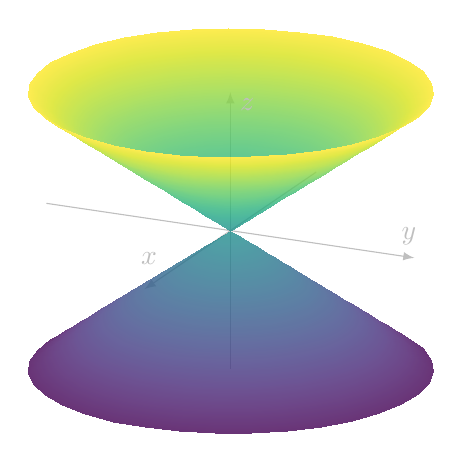
\begin{tikzpicture}
    \begin{axis}[
        axis lines = center,
        axis line style={-latex, gray!50},
        xlabel = {$x$},
        ylabel = {$y$},
        zlabel = {$z$},
        label style={gray!50},
        xmin=-2, xmax=2,
        ymin=-2, ymax=2,
        zmin=-2, zmax=2,
        ticks=none,
        view={115}{25},
        shader=interp,
        clip=false % Allows labels to breathe
    ]

        % Lower Nappe (z = -r)
        \addplot3[
            surf, 
            opacity=0.8,
            colormap/viridis, 
            domain=0:2, 
            y domain=0:360, 
            samples=25, 
            samples y=36, 
            z buffer=sort
        ] 
        ({x*cos(y)}, {x*sin(y)}, {-x});

        % Upper Nappe (z = r)
        \addplot3[
            surf, 
            opacity=0.8,
            colormap/viridis, 
            domain=0:2, 
            y domain=0:360, 
            samples=25, 
            samples y=36, 
            z buffer=sort
        ] 
        ({x*cos(y)}, {x*sin(y)}, {x});

    \end{axis}
\end{tikzpicture}
\]
Τα σύνολα αυτής της μορφής έχουν δικό τους όνομα.

\begin{definition}
    \label{def:variety}
    Το σύνολο
    \[
    \AA^n = \AA_F^n \coloneqq \{(a_1, a_2, \dots, a_n) : a_1, a_2, \dots, a_n \in F\}
    \]
    ονομάζεται \defn{αφφινικός χώρος} (affine space). Θα συμβολίζουμε τα στοιχεία του $\AA^n$ με έντονα γράμματα, δηλαδή $\bfa = (a_1, a_2, \dots, a_n)$. Για $S \subseteq \Pol{n}$, το σύνολο\footnote{Στην βιβλιογραφία συμβολίζεται και ως $\VV(\cdot)$ ή $\zZ(\cdot)$. Όταν $S = \{f\}$, θα γράφουμε απλώς $\vV(f)$.} 
    \[
    \vV(S) \coloneqq \{\bfa \in \AA^n : f(\bfa) = 0, \ \text{για κάθε $f \in S$}\}
    \]
    ονομάζεται \defn{σύνολο μηδενισμού} (zero locus) του $S$. Τα υποσύνολα του αφφινικού χώρου με αυτή την μορφή\footnote{Σε μερικά συγγράματα χρησιμοποιείται ο όρος \emph{αλγεβρικά σύνολα} γι αυτό που αποκαλούμε εμείς αφφινικές πολλαπλότητες. Στα συγγράματα αυτά, ορίζουν τις πολλαπλότητες ως ανάγωγα αλγεβρικά σύνολα, έννοια που θα συναντήσουμε στη συνέχεια.} ονομάζονται \defn{αφφινικές} (ή \defn{ομοπαραλληλικές}) \defn{πολλαπλότητες} (affine varieties).
\end{definition}

Ως σύνολο, ο αφφινικός χώρος είναι απλώς το $F^n$. Χρησιμοποιούμε διαφορετικό συμβολισμό, διότι το $F^n$ έχει δομή διανυσματικού χώρου και δακτύλιου, όπως έχουμε δει, αλγεβρικές δομές που στο $\AA^n$ θέλουμε να αγνοήσουμε. Από εδώ και στο εξής όταν λέμε πολλαπλότητα θα εννοούμε αφφινική πολλαπλότητα.

Με άλλα λόγια, μια πολλαπλότητα είναι το σύνολο λύσεων ενός συστήματος πολυωνυμικών εξισώσεων. Η αλγεβρική γεωμετρία είναι ουσιαστικά η μελέτη της γεωμετρίας των πολλαπλοτήτων. Με τον συμβολισμό του Ορισμού \ref{def:variety}, στα προηγούμενα παραδείγματα είδαμε τις πολλαπλότητες $\vV(y-x^2) \subset \AA_\RR^2$ και $\vV(x^2+y^2-z^2) \subset \AA_\RR^3$, αντίστοιχα.

\begin{remark}
    \leavevmode
    \begin{itemize}
        \item Για $S \subseteq T$, έχουμε $\vV(T) \subseteq \vV(S)$ (γιατί;). Με άλλα λόγια, όσο περισσότερες είναι οι εξισώσεις, τόσο λιγότερες είναι οι λύσεις. Για παράδειγμα, στο πραγματικό αφφινικό επίπεδο, η πολλαπλότητα $\vV(x^2+y^2-1)$ αντιστοιχεί σε έναν κύκλο, ενώ $\vV(\{x^2 + y^2 -1, x+y-2\}) = \emptyset$
        \[
        \begin{tikzpicture}
            \begin{axis}[
                axis lines = middle,
                axis line style={-latex, gray!50},
                xlabel = {$x$},
                ylabel = {$y$},
                label style={gray!50},
                % Adjusted limits to show the line clearly
                xmin=-1.5, xmax=2.5,
                ymin=-1.5, ymax=2.5,
                axis equal, 
                samples=100,
                xticklabels=\empty,
                yticklabels=\empty,
                ticks=none
                ]

            % The circle V: x^2 + y^2 - 1 = 0
            \addplot[thick, domain=0:360] ({cos(x)}, {sin(x)});
            
            % The line W: x + y - 2 = 0 => y = 2 - x
            % We choose a domain that shows where it passes the circle
            \addplot[thick, dashed, domain=-0.5:2.5] {2-x};
            \end{axis}
        \end{tikzpicture}
        \]
        \item Η πολλαπλότητα που αντιστοιχεί σε ένα σύνολο πολυωνύμων ταυτίζεται με την πολλαπλότητα που αντιστοιχεί στο ιδεώδες που παράγεται από το σύνολο αυτό. Πράγματι, έστω $S \subseteq \Pol{n}$ και $I = (S)$. Επειδή $S \subseteq I$, από την πρώτη παρατήρηση, έπεται ότι $\vV(I) \subseteq \vV(S)$. Αντιστρόφως, επειδή ένα στοιχείο του $I$ έχει την μορφή 
        \[
        g = \sum_{f \in S} p_f f 
        \]
        για κάποια $p_f \in \Pol{n}$ έπεται ότι 
        \[
        g(\bfa) = \sum_{f \in S} p_f(\bfa) \underbrace{f(\bfa)}_{= \ 0} = 0 
        \]
        για κάθε $\bfa \in \vV(S)$. Συνεπώς, $\vV(S) \subseteq \vV(I)$ και γι αυτό $\vV(I) = \vV(S)$.
    \end{itemize}
\end{remark}

\begin{example}
    \label{ex:variety}
    \leavevmode
    \begin{itemize}
        \item[(α)] Ο αφφινικός χώρος είναι πολλαπλότητα, διότι $\AA^n = \vV(\emptyset)$.
        \item[(β)] Το κενό σύνολο είναι και αυτό πολλαπλότητα, διότι $\emptyset = \vV(\Pol{n})$. 
        \item[(γ)] Για $n=1$ και $f(x) \in F[x]$, η πολλαπλότητα $\vV(f)$ είναι πεπερασμένη (γιατί;) και αποτελείται από το σύνολο όλων των ριζών του πολυωνύμου $f(x)$. Για παράδειγμα,  
        \[
        \begin{tikzpicture}
        \begin{axis}[
            axis lines = middle,
            axis line style={-latex, gray!50},
            xlabel = {$x$},
            label style={gray!50},
            % Set horizontal range as requested
            xmin=-11, xmax=3,
            % Flatten y-axis for R^1 visualization
            ymin=-0.5, ymax=0.5,
            axis y line=none, 
            % Show only the 0 tick label
            xtick={0.5},
            xticklabels={0},
            xticklabel style={gray!50},
        ]

        % Plot the three roots as blue dots
        \addplot[
            only marks,
            mark=*,
            mark size=2.5pt,
        ] 
        coordinates {
            (-9.8989, 0) 
            (-1, 0) 
            (-0.1010, 0)
        };

        \end{axis}
        \end{tikzpicture}
        \]
        $\vV(1 + 11x + 11x^2 + x^3) = \{-1, -5 \pm 2\sqrt{6}\} \subseteq \AA_\RR^1$.
    \end{itemize}
\end{example}

% \begin{thebibliography}{99}
%     \bibitem{EKPA_LA}
%     Δ. Α. Βάρσος, Δ. Ι. Δεριζιώτης, Ι. Π. Εμμανουήλ, Μ. Π. Μαλιάκας, Α. Δ. Μελάς και Ο. Π. Ταλέλλη, 
%     \emph{Μια Εισαγωγή στην Γραμμική Άλγεβρα}, 
%     Εκδόσεις Σοφία, 2012.
%     %
%     \bibitem{DF04}
%     D. S. Dummit και R. M. Foote, 
%     \textit{Abstract algebra},
%     third edition, Wiley, 2004. 
%     %
%     \bibitem{EKPA_PID}
%     Μ. Π. Μαλιάκας, και Ο. Π. Ταλέλλη, 
%     \emph{Πρότυπα πάνω από Περιοχές Κυρίων Ιδεωδών και Εφαρμογές}, 
%     Εκδόσεις Σοφία, 2009.
%     %
%     \bibitem{StaAC}
%     R. P. Stanley,
%     \emph{Algebraic Combinatorics; Walks, Trees, Tableaux and More},
%     second edition, Undergraduate Texts in Mathematics, Springer, 2018.
% \end{thebibliography}
\end{document}